\documentclass[aspectratio=169,10pt]{beamer}

\makeatletter
\NeedsTeXFormat{LaTeX2e}
\ProvidesPackage{beamerthemeDUNEProfessional}[2026/08/19 DUNE professional Beamer theme]

\mode<presentation>

\RequirePackage{iftex}
\RequirePackage{graphicx}
\RequirePackage{xcolor}
\RequirePackage{tikz}
\RequirePackage{adjustbox}
\RequirePackage{array}
\RequirePackage{booktabs}
\RequirePackage{tabularx}
\RequirePackage{ragged2e}

\usetikzlibrary{arrows.meta,calc,fit,positioning,shapes.geometric}

\useinnertheme{default}
\useoutertheme{default}
\usefonttheme{professionalfonts}
\setbeamertemplate{navigation symbols}{}

% Logo path is relative to a deck directory. Override with \DuneSetLogoPath.
\newcommand{\DuneLogoPath}{../../templates/dune-professional/logos}
\newcommand{\DuneSetLogoPath}[1]{\renewcommand{\DuneLogoPath}{#1}}

% Color roles. Keep semantic names in decks; avoid ad hoc local colors.
\definecolor{DuneBg}{HTML}{101820}
\definecolor{DunePanel}{HTML}{1B2733}
\definecolor{DunePanelAlt}{HTML}{263645}
\definecolor{DuneTitleBand}{HTML}{20303E}
\definecolor{DuneLine}{HTML}{536878}
\definecolor{DuneText}{HTML}{F1F5F7}
\definecolor{DuneMuted}{HTML}{BAC6CF}
\definecolor{DuneOrange}{HTML}{F2682B}
\definecolor{DuneCyan}{HTML}{8EDDF2}
\definecolor{DuneMint}{HTML}{9BD7AE}
\definecolor{DuneYellow}{HTML}{E8C85A}
\definecolor{DuneRed}{HTML}{F38B7F}
\definecolor{DuneViolet}{HTML}{B8A7E8}

\setbeamercolor{normal text}{fg=DuneText,bg=DuneBg}
\setbeamercolor{title}{fg=white,bg=DuneBg}
\setbeamercolor{subtitle}{fg=DuneMuted,bg=DuneBg}
\setbeamercolor{author}{fg=DuneCyan,bg=DuneBg}
\setbeamercolor{date}{fg=DuneMuted,bg=DuneBg}
\setbeamercolor{frametitle}{fg=white,bg=DuneBg}
\setbeamercolor{headline}{fg=DuneMuted,bg=DuneBg}
\setbeamercolor{footline}{fg=DuneMuted,bg=DuneBg}
\setbeamercolor{itemize item}{fg=DuneOrange}
\setbeamercolor{itemize subitem}{fg=DuneCyan}
\setbeamercolor{enumerate item}{fg=DuneOrange}
\setbeamercolor{caption name}{fg=DuneMuted}

\setbeamercolor{dune panel}{fg=DuneText,bg=DunePanel}
\setbeamercolor{dune panel alt}{fg=DuneText,bg=DunePanelAlt}
\setbeamercolor{dune accent}{fg=DuneBg,bg=DuneCyan}
\setbeamercolor{dune decision}{fg=DuneBg,bg=DuneYellow}
\setbeamercolor{dune risk}{fg=DuneBg,bg=DuneRed}
\setbeamercolor{dune evidence}{fg=DuneBg,bg=DuneMint}
\setbeamercolor{dune violet}{fg=DuneBg,bg=DuneViolet}

\setbeamerfont{normal text}{size=\small}
\setbeamerfont{title}{series=\bfseries}
\setbeamerfont{subtitle}{size=\large}
\setbeamerfont{author}{size=\normalsize,series=\bfseries}
\setbeamerfont{date}{size=\small}
\setbeamerfont{frametitle}{series=\bfseries}
\setbeamerfont{footline}{size=\scriptsize}

\ifPDFTeX
  \RequirePackage[scaled]{helvet}
  \renewcommand*\familydefault{\sfdefault}
  \RequirePackage[T1]{fontenc}
\else
  \RequirePackage{fontspec}
  \defaultfontfeatures{Ligatures=TeX,Scale=MatchLowercase}
  \IfFontExistsTF{IBM Plex Sans}{
    \setsansfont{IBM Plex Sans}
    \setmainfont{IBM Plex Sans}
  }{
    \IfFontExistsTF{Helvetica Neue}{
      \setsansfont{Helvetica Neue}
      \setmainfont{Helvetica Neue}
    }{
      \IfFontExistsTF{TeX Gyre Heros}{
        \setsansfont{TeX Gyre Heros}
        \setmainfont{TeX Gyre Heros}
      }{
        \IfFontExistsTF{Liberation Sans}{
          \setsansfont{Liberation Sans}
          \setmainfont{Liberation Sans}
        }{
          \setsansfont{DejaVu Sans}
          \setmainfont{DejaVu Sans}
        }
      }
    }
  }
  \IfFontExistsTF{JetBrains Mono}{
    \setmonofont{JetBrains Mono}[Scale=0.88]
  }{
    \IfFontExistsTF{Latin Modern Mono}{
      \setmonofont{Latin Modern Mono}[Scale=0.88]
    }{
      \setmonofont{DejaVu Sans Mono}[Scale=0.88]
    }
  }
  \renewcommand*\familydefault{\sfdefault}
\fi

\setbeamersize{text margin left=0.78cm,text margin right=0.78cm}
\setlength{\leftmargini}{1.15em}
\setlength{\leftmarginii}{1.05em}
\setlength{\parskip}{0.18em}

\setbeamertemplate{itemize item}{%
  \color{DuneOrange}\raisebox{0.15ex}{\scriptsize$\blacktriangleright$}%
}
\setbeamertemplate{itemize subitem}{%
  \color{DuneCyan}\raisebox{0.15ex}{\tiny$\blacktriangleright$}%
}

% Measured boxes: content may shrink down, but never expands outside the safe box.
\newcommand{\DuneFitBox}[3]{%
  \begin{adjustbox}{max width=#1,max totalheight=#2}%
    \begin{minipage}{#1}\raggedright #3\end{minipage}%
  \end{adjustbox}%
}

\newcommand{\DuneTightList}{%
  \setlength{\itemsep}{0.45mm}%
  \setlength{\parskip}{0pt}%
}

\newcommand{\DuneEyebrow}[1]{%
  {\color{DuneCyan}\scriptsize\bfseries #1\par}%
}

\newcommand{\DunePill}[2]{%
  \tikz[baseline=-0.55ex]\node[
    rounded corners=2.5pt,
    draw=#1,
    fill=#1!18!DuneBg,
    inner xsep=4pt,
    inner ysep=1.35pt,
    text=#1,
    font=\tiny\bfseries
  ]{#2};%
}

\newcommand{\DuneCard}[4][dune panel]{%
  \begin{beamercolorbox}[wd=\linewidth,sep=5pt,rounded=true]{#1}
    {\usebeamercolor[fg]{#1}\bfseries #2\par}
    \vspace{0.4mm}
    {\usebeamercolor[fg]{#1}\footnotesize #3\par}
    \if\relax\detokenize{#4}\relax\else
      \vspace{0.5mm}{\usebeamercolor[fg]{#1}\scriptsize #4\par}
    \fi
  \end{beamercolorbox}
}

\newcommand{\DuneFixedCard}[5][dune panel]{%
  \begin{beamercolorbox}[wd=\linewidth,sep=5pt,rounded=true]{#1}
    \begin{minipage}[t][#2][t]{\dimexpr\linewidth-10pt\relax}
      \raggedright
      {\usebeamercolor[fg]{#1}\bfseries #3\par}
      \vspace{0.45mm}
      {\usebeamercolor[fg]{#1}\footnotesize #4\par}
      \if\relax\detokenize{#5}\relax\else
        \vspace{0.55mm}{\usebeamercolor[fg]{#1}\scriptsize #5\par}
      \fi
    \end{minipage}
  \end{beamercolorbox}
}

\newcommand{\DuneFooterLogo}{%
  \IfFileExists{\DuneLogoPath/logosolo.png}{%
    \tikz[baseline=-0.52ex]\node[opacity=0.42,inner sep=0pt]{%
      \includegraphics[height=0.25cm]{\DuneLogoPath/logosolo.png}%
    };%
  }{}%
}

\newcommand{\DuneTalkDate}{%
  \@ifundefined{mydate}{\today}{\mydate}%
}

% Background and fixed frame-title band.
\addtobeamertemplate{background canvas}{%
  \begin{tikzpicture}[remember picture,overlay]
    \fill[DuneBg] (current page.south west) rectangle (current page.north east);
    \draw[DuneLine,line width=0.55pt]
      ($(current page.south west)+(0.78,0.74)$)
      -- ($(current page.south east)+(-0.78,0.74)$);
    \fill[DuneCyan!16]
      ($(current page.south east)+(-3.2,0.83)$) rectangle ++(1.45,0.055);
  \end{tikzpicture}%
}{}

\setbeamertemplate{headline}{}

\setbeamertemplate{frametitle}{%
  \nointerlineskip%
  \begin{tikzpicture}[remember picture,overlay]
    \fill[DuneTitleBand]
      (current page.north west) rectangle ($(current page.north east)+(0,-1.18)$);
    \fill[DuneOrange]
      ($(current page.north west)+(0.78,-0.23)$) rectangle ++(1.38,0.055);
    \node[anchor=west,inner sep=0pt]
      at ($(current page.north west)+(0.78,-0.72)$) {%
        \DuneFitBox{\dimexpr\paperwidth-1.56cm\relax}{6.7mm}{%
          {\color{white}\bfseries\fontsize{17}{20}\selectfont\insertframetitle}%
        }%
      };
    \ifx\insertframesubtitle\@empty\else
      \node[anchor=west,inner sep=0pt]
        at ($(current page.north west)+(0.78,-1.02)$) {%
          \DuneFitBox{\dimexpr\paperwidth-1.56cm\relax}{3.2mm}{%
            {\color{DuneMuted}\scriptsize\insertframesubtitle}%
          }%
        };
    \fi
  \end{tikzpicture}%
  \vspace*{12.5mm}%
}

\setbeamertemplate{footline}{%
  \leavevmode%
  \begin{beamercolorbox}[wd=\paperwidth,ht=6.4mm,dp=1.8mm,leftskip=0.78cm,rightskip=0.78cm]{footline}
    \DuneFooterLogo\hspace{0.45em}{\textcolor{DuneMuted}{\DuneTalkDate}}%
    \hfill%
    {\textcolor{DuneOrange}{\bfseries\insertframenumber}\textcolor{DuneMuted}{/\inserttotalframenumber}}%
  \end{beamercolorbox}%
}

\setbeamertemplate{title page}{%
  \begin{tikzpicture}[remember picture,overlay]
    \fill[DuneBg] (current page.south west) rectangle (current page.north east);
    \fill[DuneTitleBand]
      (current page.north west) rectangle ($(current page.north east)+(0,-3.03)$);
    \fill[DuneOrange]
      ($(current page.north west)+(0.82,-0.58)$) rectangle ++(1.55,0.075);
    \fill[DuneCyan]
      ($(current page.south east)+(-2.8,0.79)$) rectangle ++(1.88,0.065);
    \IfFileExists{\DuneLogoPath/DUNElogo_white.png}{%
      \node[anchor=south east,opacity=0.13,inner sep=0pt]
        at ($(current page.south east)+(-0.55,1.42)$) {%
        \includegraphics[width=0.34\paperwidth]{\DuneLogoPath/DUNElogo_white.png}%
      };
    }{}%
    \IfFileExists{\DuneLogoPath/FNAL-Logo-NAL-Light.png}{%
      \node[anchor=south east,inner sep=0pt]
        at ($(current page.south east)+(-0.92,0.78)$) {%
        \includegraphics[height=0.42cm]{\DuneLogoPath/FNAL-Logo-NAL-Light.png}%
      };
    }{}%
    \node[anchor=north west,inner sep=0pt]
      at ($(current page.north west)+(0.82,-0.88)$) {%
        \DuneFitBox{0.78\paperwidth}{1.48cm}{%
          {\color{white}\bfseries\fontsize{25}{28}\selectfont\inserttitle}%
        }%
      };
    \node[anchor=north west,inner sep=0pt]
      at ($(current page.north west)+(0.82,-3.55)$) {%
        \DuneFitBox{0.56\paperwidth}{1.35cm}{%
          {\color{DuneMuted}\fontsize{13}{17}\selectfont\insertsubtitle}%
        }%
      };
    \node[anchor=north west,text=DuneCyan,font=\bfseries,inner sep=0pt]
      at ($(current page.north west)+(0.82,-6.3)$) {\insertauthor};
    \node[anchor=north west,text=DuneMuted,font=\small,inner sep=0pt]
      at ($(current page.north west)+(0.82,-6.82)$) {\insertdate};
  \end{tikzpicture}%
  \vfill%
}

\tikzset{
  dune repo/.style={
    draw=DuneCyan,
    fill=DuneCyan!12!DunePanel,
    text=DuneText,
    rounded corners=3pt,
    align=center,
    text width=2.35cm,
    minimum height=0.86cm,
    inner sep=4pt,
    font=\scriptsize\bfseries
  },
  dune repo muted/.style={
    draw=DuneLine,
    fill=DunePanelAlt,
    text=DuneText,
    rounded corners=3pt,
    align=center,
    text width=2.35cm,
    minimum height=0.86cm,
    inner sep=4pt,
    font=\scriptsize\bfseries
  },
  dune artifact/.style={
    draw=DuneMint,
    fill=DuneMint!13!DunePanel,
    text=DuneText,
    rounded corners=3pt,
    align=center,
    text width=2.35cm,
    minimum height=0.86cm,
    inner sep=4pt,
    font=\scriptsize\bfseries
  },
  dune decision node/.style={
    draw=DuneYellow,
    fill=DuneYellow!14!DunePanel,
    text=DuneText,
    rounded corners=3pt,
    align=center,
    text width=2.35cm,
    minimum height=0.86cm,
    inner sep=4pt,
    font=\scriptsize\bfseries
  },
  dune flow/.style={-Latex,draw=DuneCyan,line width=0.85pt},
  dune relation/.style={draw=DuneMuted,line width=0.65pt},
  dune evidence flow/.style={-Latex,draw=DuneViolet,dashed,line width=0.85pt},
  dune label/.style={
    fill=DuneBg,
    text=DuneMuted,
    inner sep=1.5pt,
    font=\tiny,
    align=center
  }
}

\mode<all>

\makeatother

\usepackage{amsmath}
\usepackage{multirow}

\title[SC/DPS Repository Plan]{SC/DPS Repository Plan}
\subtitle{A governed collection for slow-controls software, contracts, bridges, emulators, and deployment}
\author{Manuel Arroyave}
\date{DUNE slow-controls software discussion -- 20 August 2026}
\newcommand{\mydate}{20 August 2026}

\begin{document}

\begin{frame}[plain]
  \titlepage
\end{frame}

\begin{frame}{Decision for Thursday}
\begin{columns}[T,onlytextwidth]
  \begin{column}{0.56\textwidth}
    \DuneEyebrow{ASK FOR AGREEMENT}
    \begin{itemize}
      \DuneTightList
      \item Use an official DUNE-controlled namespace or an equivalent governed collection.
      \item Keep existing DUNE DAQ and firmware repositories as first-class members.
      \item Assign one canonical source for each schema, descriptor, and interface contract.
      \item Start with two vertical pilots: board-to-OPC-UA and rack-power/DPS permit.
      \item Exclude secrets, site endpoints, certificates, Gateway backups, and private configuration.
    \end{itemize}
  \end{column}
  \begin{column}{0.40\textwidth}
    \DuneFixedCard[dune decision]{1.35cm}{Recommendation}
      {A small repository collection, not a monorepo and not untracked personal forks.}
      {}
    \vspace{1.5mm}
    \DuneFixedCard[dune evidence]{1.35cm}{Naming}
      {\texttt{scdps-*} for system-level repositories; \texttt{<device>-<role>} for device implementations.}
      {}
    \vspace{1.5mm}
    \DuneFixedCard[dune panel alt]{1.35cm}{Near-term outcome}
      {A repository catalog, owner list, branch policy, and migration checklist before wider onboarding.}
      {}
  \end{column}
\end{columns}
\end{frame}

\begin{frame}{Repository Relationship Topology}
\centering
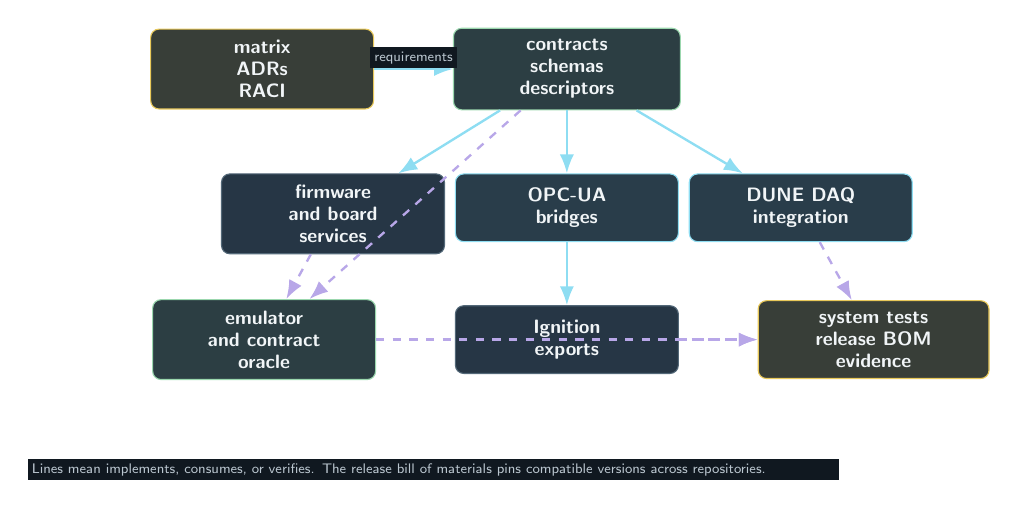
\begin{tikzpicture}[node distance=8mm and 10mm]
  \node[dune decision node,text width=2.55cm] (coord) {matrix\\ADRs\\RACI};
  \node[dune artifact,text width=2.6cm,right=of coord] (contracts) {contracts\\schemas\\descriptors};
  \node[dune repo muted,text width=2.55cm,below left=8mm and 1mm of contracts] (firmware) {firmware\\and board\\services};
  \node[dune repo,text width=2.55cm,below=of contracts] (bridges) {OPC-UA\\bridges};
  \node[dune repo,text width=2.55cm,below right=8mm and 1mm of contracts] (daq) {DUNE DAQ\\integration};
  \node[dune repo muted,text width=2.55cm,below=of bridges] (ignition) {Ignition\\exports};
  \node[dune artifact,text width=2.55cm,left=of ignition] (emulator) {emulator\\and contract\\oracle};
  \node[dune decision node,text width=2.65cm,right=of ignition] (tests) {system tests\\release BOM\\evidence};

  \draw[dune flow] (coord) -- node[dune label,above] {requirements} (contracts);
  \draw[dune flow] (contracts) -- (firmware);
  \draw[dune flow] (contracts) -- (bridges);
  \draw[dune flow] (contracts) -- (daq);
  \draw[dune flow] (bridges) -- (ignition);
  \draw[dune evidence flow] (contracts) -- (emulator);
  \draw[dune evidence flow] (firmware) -- (emulator);
  \draw[dune evidence flow] (emulator) -- (tests);
  \draw[dune evidence flow] (daq) -- (tests);
  \draw[dune evidence flow] (ignition) -- (tests);

  \node[dune label,align=left,text width=10.2cm,below=10mm of emulator,xshift=2.15cm] {
    Lines mean implements, consumes, or verifies. The release bill of materials pins compatible versions across repositories.
  };
\end{tikzpicture}
\end{frame}

\begin{frame}{Proposed Repository Collection}
\scriptsize
\renewcommand{\arraystretch}{1.15}
\begin{tabularx}{\textwidth}{>{\bfseries\ttfamily}p{0.24\textwidth} X p{0.30\textwidth}}
\toprule
Repo & Owns & Seed from current work \\
\midrule
scdps-coordination &
Interaction matrix, ADRs, RACI, risks, source register, release compatibility table. &
\texttt{daphne\_slow\_controls\_plan} \\
\addlinespace
scdps-contracts &
Shared status, quality, provenance, authority, schema policy, descriptor hashes. &
Extract from DAPHNE/WIB/GIZMo after interface review. \\
\addlinespace
scdps-interfaces &
ICD sources, intake workbooks, public review packages, controlled-source register. &
\texttt{sc\_interface}, \texttt{gizmo-icd} \\
\addlinespace
scdps-emulator &
Fleet emulator, protocol adapters, scenarios, fault injection, contract oracle. &
\texttt{detector-control-emulator} / \texttt{sc\_emu} \\
\addlinespace
scdps-bridge-core &
Reusable OPC-UA service shell, cache/quality/staleness, metrics, audit, config. &
Reusable pieces from DAPHNE bridge work. \\
\addlinespace
daphne-opcua-bridge, wib-opcua-bridge &
Device-specific mappings, methods, tests, and source protocol pinning. &
\texttt{daphne-sc/opcua-bridge}, \texttt{wib\_opcua} \\
\addlinespace
scdps-deployment, scdps-system-tests &
Host roles, service/container definitions, release BOM, rollback, VST evidence. &
Reviewed deployment files plus emulator harness. \\
\bottomrule
\end{tabularx}
\end{frame}

\begin{frame}{Naming and Ownership Rules}
\begin{columns}[T,onlytextwidth]
  \begin{column}{0.48\textwidth}
    \DuneFixedCard[dune accent]{1.95cm}{System-level repositories}
      {\texttt{scdps-coordination}\\\texttt{scdps-contracts}\\\texttt{scdps-emulator}\\\texttt{scdps-deployment}}
      {Owned by the SC/DPS collaboration team with CODEOWNERS for specific areas.}
    \vspace{1.5mm}
    \DuneFixedCard[dune evidence]{1.95cm}{Device-level repositories}
      {\texttt{daphne-opcua-bridge}\\\texttt{wib-opcua-bridge}\\\texttt{gizmo-runtime}}
      {Owned by the responsible device or subsystem team.}
  \end{column}
  \begin{column}{0.48\textwidth}
    \DuneEyebrow{RULES THAT PREVENT CONFUSION}
    \begin{itemize}
      \DuneTightList
      \item Repo name states the ownership boundary, not the implementation language.
      \item Contracts are versioned artifacts, not scattered copies in every client.
      \item Public by default; controlled deployment values live outside Git.
      \item Personal forks remain development spaces, not collaboration sources of record.
      \item System releases pin exact compatible versions across repositories.
    \end{itemize}
  \end{column}
\end{columns}
\end{frame}

\begin{frame}{Onboard Existing Work Without a Restart}
\centering
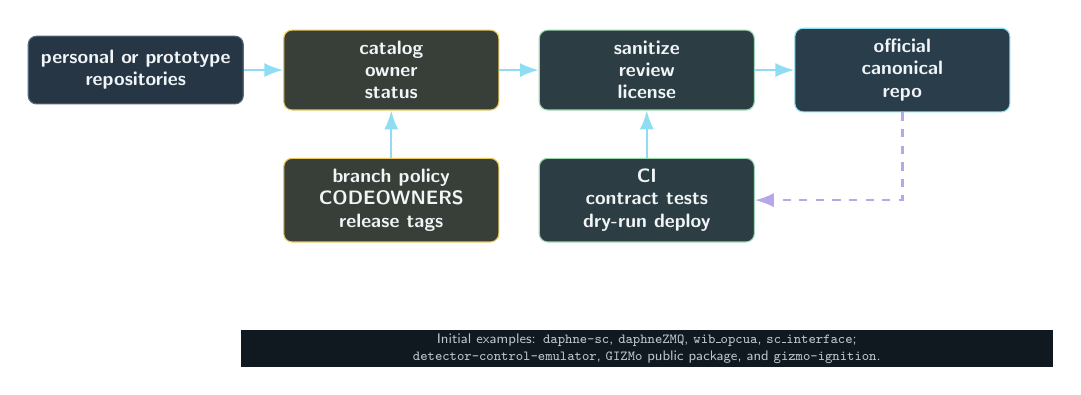
\begin{tikzpicture}[node distance=6mm and 5mm]
  \node[dune repo muted,text width=2.45cm] (personal) {personal or prototype\\repositories};
  \node[dune decision node,text width=2.45cm,right=of personal] (catalog) {catalog\\owner\\status};
  \node[dune artifact,text width=2.45cm,right=of catalog] (review) {sanitize\\review\\license};
  \node[dune repo,text width=2.45cm,right=of review] (official) {official\\canonical\\repo};
  \node[dune decision node,text width=2.45cm,below=of catalog] (policy) {branch policy\\CODEOWNERS\\release tags};
  \node[dune artifact,text width=2.45cm,below=of review] (ci) {CI\\contract tests\\dry-run deploy};

  \draw[dune flow] (personal) -- (catalog);
  \draw[dune flow] (catalog) -- (review);
  \draw[dune flow] (review) -- (official);
  \draw[dune flow] (policy) -- (catalog);
  \draw[dune flow] (ci) -- (review);
  \draw[dune evidence flow] (official) |- (ci);

  \node[dune label,text width=10.2cm,align=center,below=11mm of ci] {
    Initial examples: \texttt{daphne-sc}, \texttt{daphneZMQ}, \texttt{wib\_opcua}, \texttt{sc\_interface};\\
    \texttt{detector-control-emulator}, \texttt{GIZMo} public package, and \texttt{gizmo-ignition}.
  };
\end{tikzpicture}
\end{frame}

\begin{frame}{First Vertical Pilots}
\begin{columns}[T,onlytextwidth]
  \begin{column}{0.48\textwidth}
    \DuneFixedCard[dune evidence]{2.65cm}{Pilot 1: board to OPC-UA}
      {DAPHNE/WIB status and readiness projected through canonical device contracts into OPC-UA, then checked against DAQ views.}
      {\DunePill{DuneMint}{read-only first}\hspace{1mm}\DunePill{DuneCyan}{schema hash}}
  \end{column}
  \begin{column}{0.48\textwidth}
    \DuneFixedCard[dune risk]{2.65cm}{Pilot 2: rack-power and permit}
      {PDU, supply, sensor, and DPS-permit path exercised through emulator scenarios and one representative hardware path.}
      {\DunePill{DuneRed}{failure survives bridge loss}\hspace{1mm}\DunePill{DuneYellow}{reset owner}}
  \end{column}
\end{columns}
\vspace{4mm}
\DuneCard[dune panel alt]{Crossing fault}
  {Inject one scenario that touches both pilots: permit loss during DAQ configure or SC command. The result should be visible in DAQ, OPC-UA/Ignition, and the evidence report, without crediting monitoring software for independent protection.}
  {}
\end{frame}

\begin{frame}{Governance Minimum for the First Repos}
\begin{columns}[T,onlytextwidth]
  \begin{column}{0.50\textwidth}
    \begin{itemize}
      \DuneTightList
      \item Protected default and release branches.
      \item No direct pushes to protected branches.
      \item Required status checks for build, tests, and contract compatibility.
      \item Traceable release tags and retained artifacts.
      \item CODEOWNERS for schemas, firmware ABI, protection logic, deployment, and matrix rows.
    \end{itemize}
  \end{column}
  \begin{column}{0.46\textwidth}
    \DuneFixedCard[dune decision]{1.35cm}{Meeting output}
      {Choose namespace, first repo names, maintainers, and migration order.}
      {}
    \vspace{1.5mm}
    \DuneFixedCard[dune panel alt]{1.35cm}{Do not decide yet}
      {Do not force every prototype to move before the catalog and review gates exist.}
      {}
    \vspace{1.5mm}
    \DuneFixedCard[dune evidence]{1.35cm}{Concrete next step}
      {Create \texttt{scdps-coordination} and merge the repository catalog plus decision record.}
      {}
  \end{column}
\end{columns}
\end{frame}

\end{document}
